El modelado de los sistemas y relaciones entre variables es una tarea fundamental en m\'ultiples \'areas.
Los sistemas pueden definirse como una relaci\'on entre variables de entrada y salida, donde la salida es una funci\'on de las entradas $y = f(x)$. \\

\begin{figure}[H]
    \centering
    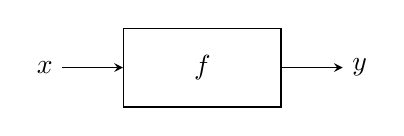
\begin{tikzpicture}
        \node (input) at (0, 0) [] {$x$};
        \node (output) at (4, 0) [] {$y$};
        \node[rectangle,, draw, minimum width=2cm, minimum height=1cm] (system) at (2, 0) {$f$};
        \draw[-stealth] (input) -- (system);
        \draw[-stealth] (system) -- (output);
    \end{tikzpicture}
    \caption{Sistema a modelar}
\end{figure}


Ahora, lo que se busca al modelar es obtener una funci\'on $\hat{f}$ que aproxime a $f$ de la \say{mejor manera posible}\footnote{Veremos el significado de esto en la secci\'on COMPLETAR}, $\hat{y} = \hat{f}(x)$. \\

\begin{figure}[H]
    \centering
    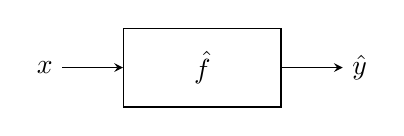
\begin{tikzpicture}
        \node (input) at (0, 0) [] {$x$};
        \node (output) at (4, 0) [] {$\hat{y}$};
        \node[rectangle,, draw, minimum width=2cm, minimum height=1cm] (system) at (2, 0) {$\hat{f}$};
        \draw[-stealth] (input) -- (system);
        \draw[-stealth] (system) -- (output);
    \end{tikzpicture}
    \caption{Modelo del sistema}
\end{figure}

La pregunta a responder es ¿cómo obtener $\hat{f}$?. Para simplificar, supongamos que tenemos un sistema que podemos modelar mediante una regresion lineal, es decir aproximemos $f$ con una recta. \\

\begin{equation}
    \hat{y} = \mathbf{w} x + \mathbf{b}
\end{equation}

Donde $\mathbf{w}$ y $\mathbf{b}$ son los par\'ametros del modelo. Estos par\'ametros son los que se deben ajustar para que $\hat{f}$ se aproxime lo \say{mejor posible} a $f$. \\

La forma de ajustar estos par\'ametros es a partir de un conjunto de datos de entrada y salida de la forma $\left(x_i, y_i\right)$. Es decir, tenemos una serie de entradas conocidas $X$ y sus respectivas salidas $Y$, y a partir de estos datos \textit{etiquetados} se busca ajustar los par\'ametros del modelo. \\

Se buscaran los par\'ametros $\mathbf{w}$, $\mathbf{b}$ que minimicen alguna m\'etrica de error, definida por una funci\'on de costo, la cual determina que significa \say{mejor posible}. \\

En el caso de una regresi\'on lineal, la funci\'on de costo m\'as com\'un es el error cuadr\'atico medio (MSE). Es decir que se busca minimizar la siguiente funci\'on:

\begin{equation}
    \text{MSE} = \frac{1}{n} \sum_{i=1}^{n} \left(y_i - \hat{y}_i\right)^2
\end{equation}

Donde $n$ es la cantidad de datos de entrenamiento.\\

Es posible deducir de manera anal\'itica los valores de $\mathbf{w}$ y $\mathbf{b}$ que minimizan la funci\'on de costo. Para esto, se deriva la funci\'on de costo con respecto a los par\'ametros y se iguala a cero. Lo cual nos lleva a las siguientes soluciones:

\begin{equation}
    \begin{split}
        \mathbf{w} &= \left(X^T X\right)^{-1} X^T \mathbf{y} \\
        \mathbf{b} &= \bar{y} - \mathbf{w} \bar{x}
    \end{split}
\end{equation}

Sin embargo, en la pr\'actica, el c\'alculo de estas soluciones puede ser computacionalmente costoso, especialmente cuando la cantidad de datos es muy grande. Computar la inversa de una matriz es un proceso de orden c\'ubico en la cantidad de datos. Volveremos a este ejemplo en la secci\'on \ref{sec:redes_neuronales}. \\
